\chapter{Teoría de juegos}

En este capítulo, nos centraremos en juegos de dos jugadores
que no contienen elementos aleatorios.
Nuestro objetivo es encontrar una estrategia que podamos
seguir para ganar el juego
sin importar lo que haga el oponente,
si existe tal estrategia.

Resulta que existe una estrategia general
para tales juegos,
y podemos analizar los juegos utilizando la \key{teoría del nim}.
Primero, analizaremos juegos simples donde
los jugadores eliminan palos de pilas,
y después de esto, generalizaremos la estrategia
utilizada en esos juegos a otros juegos.

\section{Estados del juego}

Consideremos un juego donde inicialmente hay
una pila de $n$ palos.
Los jugadores $A$ y $B$ se mueven alternativamente,
y el jugador $A$ comienza.
En cada movimiento, el jugador tiene que eliminar
1, 2 o 3 palos de la pila,
y el jugador que elimina el último palo gana el juego.

Por ejemplo, si $n=10$, el juego puede proceder de la siguiente manera:
\begin{itemize}[noitemsep]
\item El jugador $A$ elimina 2 palos (quedan 8 palos).
\item El jugador $B$ elimina 3 palos (quedan 5 palos).
\item El jugador $A$ elimina 1 palo (quedan 4 palos).
\item El jugador $B$ elimina 2 palos (quedan 2 palos).
\item El jugador $A$ elimina 2 palos y gana.
\end{itemize}

Este juego consiste en estados $0,1,2,\ldots,n$,
donde el número del estado corresponde a
la cantidad de palos restantes.

\subsubsection{Estados ganadores y perdedores}

\index{estado ganador}
\index{estado perdedor}

Un \key{estado ganador} es un estado donde
el jugador ganará el juego si
juega de manera óptima,
y un \key{estado perdedor} es un estado
donde el jugador perderá el juego si el
oponente juega de manera óptima.
Resulta que podemos clasificar todos los estados
de un juego de modo que cada estado sea o bien
un estado ganador o un estado perdedor.

En el juego anterior, el estado 0 es claramente un
estado perdedor, porque el jugador no puede hacer
ningún movimiento.
Los estados 1, 2 y 3 son estados ganadores,
porque podemos eliminar 1, 2 o 3 palos
y ganar el juego.
El estado 4, a su vez, es un estado perdedor,
porque cualquier movimiento conduce a un estado que
es un estado ganador para el oponente.

Más generalmente, si hay un movimiento que conduce
desde el estado actual a un estado perdedor,
el estado actual es un estado ganador,
y de lo contrario el estado actual es un estado perdedor.
Usando esta observación, podemos clasificar todos los estados
de un juego comenzando con estados perdedores donde
no hay movimientos posibles.

Los estados $0 \ldots 15$ del juego anterior
se pueden clasificar de la siguiente manera
($W$ denota un estado ganador y $L$ denota un estado perdedor):
\begin{center}
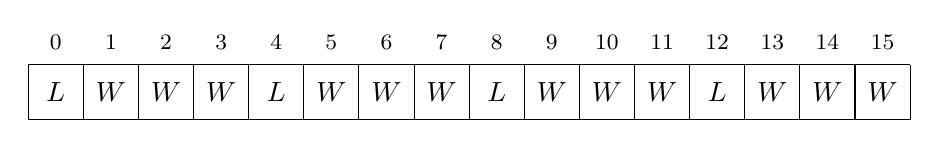
\begin{tikzpicture}[scale=0.7]
\draw (0,0) grid (16,1);

\node at (0.5,0.5) {$L$};
\node at (1.5,0.5) {$W$};
\node at (2.5,0.5) {$W$};
\node at (3.5,0.5) {$W$};
\node at (4.5,0.5) {$L$};
\node at (5.5,0.5) {$W$};
\node at (6.5,0.5) {$W$};
\node at (7.5,0.5) {$W$};
\node at (8.5,0.5) {$L$};
\node at (9.5,0.5) {$W$};
\node at (10.5,0.5) {$W$};
\node at (11.5,0.5) {$W$};
\node at (12.5,0.5) {$L$};
\node at (13.5,0.5) {$W$};
\node at (14.5,0.5) {$W$};
\node at (15.5,0.5) {$W$};

\footnotesize
\node at (0.5,1.4) {$0$};
\node at (1.5,1.4) {$1$};
\node at (2.5,1.4) {$2$};
\node at (3.5,1.4) {$3$};
\node at (4.5,1.4) {$4$};
\node at (5.5,1.4) {$5$};
\node at (6.5,1.4) {$6$};
\node at (7.5,1.4) {$7$};
\node at (8.5,1.4) {$8$};
\node at (9.5,1.4) {$9$};
\node at (10.5,1.4) {$10$};
\node at (11.5,1.4) {$11$};
\node at (12.5,1.4) {$12$};
\node at (13.5,1.4) {$13$};
\node at (14.5,1.4) {$14$};
\node at (15.5,1.4) {$15$};
\end{tikzpicture}
\end{center}

Es fácil analizar este juego:
un estado $k$ es un estado perdedor si $k$ es
divisible por 4, y de lo contrario es
un estado ganador.
Una forma óptima de jugar el juego es
siempre elegir un movimiento después del cual
la cantidad de palos en la pila
sea divisible por 4.
Finalmente, no quedan palos y
el oponente ha perdido.

Por supuesto, esta estrategia requiere que
la cantidad de palos \emph{no} sea divisible por 4
cuando es nuestro movimiento.
Si lo es, no hay nada que podamos hacer,
y el oponente ganará el juego si
juega de manera óptima.

\subsubsection{Gráfico de estado}

Consideremos ahora otro juego de palos,
donde en cada estado $k$, se permite eliminar
cualquier número $x$ de palos tal que $x$
sea menor que $k$ y divida $k$.
Por ejemplo, en el estado 8 podemos eliminar
1, 2 o 4 palos, pero en el estado 7 el único
movimiento permitido es eliminar 1 palo.

La siguiente imagen muestra los estados
$1 \ldots 9$ del juego como un \key{gráfico de estado},
cuyos nodos son los estados y las aristas son los movimientos entre ellos:

\begin{center}
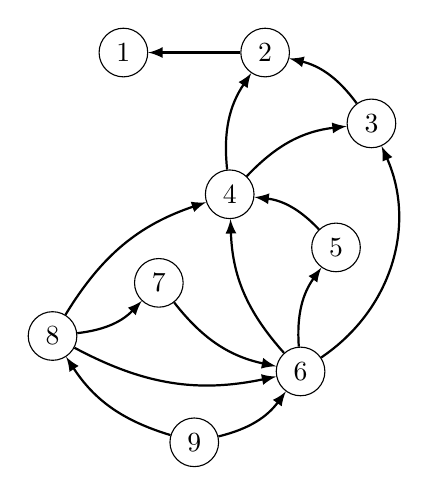
\begin{tikzpicture}[scale=0.9]
\node[draw, circle] (1) at (0,0) {$1$};
\node[draw, circle] (2) at (2,0) {$2$};
\node[draw, circle] (3) at (3.5,-1) {$3$};
\node[draw, circle] (4) at (1.5,-2) {$4$};
\node[draw, circle] (5) at (3,-2.75) {$5$};
\node[draw, circle] (6) at (2.5,-4.5) {$6$};
\node[draw, circle] (7) at (0.5,-3.25) {$7$};
\node[draw, circle] (8) at (-1,-4) {$8$};
\node[draw, circle] (9) at (1,-5.5) {$9$};

\path[draw,thick,->,>=latex] (2) -- (1);
\path[draw,thick,->,>=latex] (3) edge [bend right=20] (2);
\path[draw,thick,->,>=latex] (4) edge [bend left=20] (2);
\path[draw,thick,->,>=latex] (4) edge [bend left=20] (3);
\path[draw,thick,->,>=latex] (5) edge [bend right=20] (4);
\path[draw,thick,->,>=latex] (6) edge [bend left=20] (5);
\path[draw,thick,->,>=latex] (6) edge [bend left=20] (4);
\path[draw,thick,->,>=latex] (6) edge [bend right=40] (3);
\path[draw,thick,->,>=latex] (7) edge [bend right=20] (6);
\path[draw,thick,->,>=latex] (8) edge [bend right=20] (7);
\path[draw,thick,->,>=latex] (8) edge [bend right=20] (6);
\path[draw,thick,->,>=latex] (8) edge [bend left=20] (4);
\path[draw,thick,->,>=latex] (9) edge [bend left=20] (8);
\path[draw,thick,->,>=latex] (9) edge [bend right=20] (6);
\end{tikzpicture}
\end{center}

El estado final en este juego es siempre el estado 1,
que es un estado perdedor, porque no hay
movimientos válidos.
La clasificación de los estados $1 \ldots 9$
es la siguiente:

\begin{center}
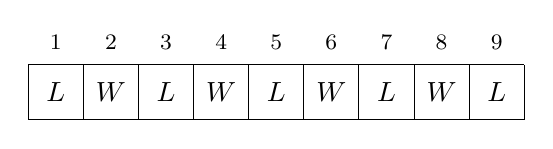
\begin{tikzpicture}[scale=0.7]
\draw (1,0) grid (10,1);

\node at (1.5,0.5) {$L$};
\node at (2.5,0.5) {$W$};
\node at (3.5,0.5) {$L$};
\node at (4.5,0.5) {$W$};
\node at (5.5,0.5) {$L$};
\node at (6.5,0.5) {$W$};
\node at (7.5,0.5) {$L$};
\node at (8.5,0.5) {$W$};
\node at (9.5,0.5) {$L$};

\footnotesize
\node at (1.5,1.4) {$1$};
\node at (2.5,1.4) {$2$};
\node at (3.5,1.4) {$3$};
\node at (4.5,1.4) {$4$};
\node at (5.5,1.4) {$5$};
\node at (6.5,1.4) {$6$};
\node at (7.5,1.4) {$7$};
\node at (8.5,1.4) {$8$};
\node at (9.5,1.4) {$9$};
\end{tikzpicture}
\end{center}

Sorprendentemente, en este juego,
todos los estados con número par son estados ganadores,
y todos los estados con número impar son estados perdedores.

\section{Juego de Nim}

\index{juego de nim}

El \key{juego de nim} es un juego simple que
tiene un papel importante en la teoría de juegos,
porque muchos otros juegos se pueden jugar usando
la misma estrategia.
Primero, nos centramos en nim,
y luego generalizamos la estrategia
a otros juegos.

Hay $n$ montones en nim,
y cada montón contiene un número de palitos.
Los jugadores se mueven alternativamente,
y en cada turno, el jugador elige
un montón que aún contiene palitos
y elimina cualquier número de palitos de él.
El ganador es el jugador que elimina el último palito.

Los estados en nim son de la forma
$[x_1,x_2,\ldots,x_n]$,
donde $x_k$ denota el número de palitos en el montón $k$.
Por ejemplo, $[10,12,5]$ es un juego donde
hay tres montones con 10, 12 y 5 palitos.
El estado $[0,0,\ldots,0]$ es un estado perdedor,
porque no es posible eliminar ningún palito,
y este es siempre el estado final.

\subsubsection{Análisis}
\index{suma de nim}

Resulta que podemos clasificar fácilmente
cualquier estado nim calculando
la \key{suma de nim} $s = x_1 \oplus x_2 \oplus \cdots \oplus x_n$,
donde $\oplus$ es la operación xor\footnote{La estrategia óptima
para nim fue publicada en 1901 por C. L. Bouton \cite{bou01}.}.
Los estados cuya suma de nim es 0 son estados perdedores,
y todos los demás estados son estados ganadores.
Por ejemplo, la suma de nim de
$[10,12,5]$ es $10 \oplus 12 \oplus 5 = 3$,
por lo que el estado es un estado ganador.

¿Pero cómo se relaciona la suma de nim con el juego nim?
Podemos explicar esto viendo cómo cambia la suma de nim
cuando cambia el estado nim.

\textit{Estados perdedores:}
El estado final $[0,0,\ldots,0]$ es un estado perdedor,
y su suma de nim es 0, como se esperaba.
En otros estados perdedores, cualquier movimiento lleva a
un estado ganador, porque cuando un solo valor $x_k$ cambia,
la suma de nim también cambia, por lo que la suma de nim
es diferente de 0 después del movimiento.

\textit{Estados ganadores:}
Podemos movernos a un estado perdedor si
hay algún montón $k$ para el cual $x_k \oplus s < x_k$.
En este caso, podemos eliminar palitos de
el montón $k$ de modo que contenga $x_k \oplus s$ palitos,
lo que conducirá a un estado perdedor.
Siempre hay un montón así, donde $x_k$
tiene un bit uno en la posición del bit uno más a la izquierda
de $s$.

Como ejemplo, considere el estado $[10,12,5]$.
Este estado es un estado ganador,
porque su suma de nim es 3.
Por lo tanto, tiene que haber un movimiento que
conduzca a un estado perdedor.
A continuación, averiguaremos tal movimiento.

La suma de nim del estado es la siguiente:

\begin{center}
\begin{tabular}{r|r}
10 & \texttt{1010} \\
12 & \texttt{1100} \\
5 & \texttt{0101} \\
\hline
3 & \texttt{0011} \\
\end{tabular}
\end{center}

En este caso, el montón con 10 palitos
es el único montón que tiene un bit uno
en la posición del bit uno más a la izquierda
de la suma de nim:

\begin{center}
\begin{tabular}{r|r}
10 & \texttt{10\underline{1}0} \\
12 & \texttt{1100} \\
5 & \texttt{0101} \\
\hline
3 & \texttt{00\underline{1}1} \\
\end{tabular}
\end{center}

El nuevo tamaño del montón tiene que ser
$10 \oplus 3 = 9$,
por lo que eliminaremos solo un palito.
Después de esto, el estado será $[9,12,5]$,
que es un estado perdedor:

\begin{center}
\begin{tabular}{r|r}
9 & \texttt{1001} \\
12 & \texttt{1100} \\
5 & \texttt{0101} \\
\hline
0 & \texttt{0000} \\
\end{tabular}
\end{center}

\subsubsection{Juego Misère}

\index{juego misère}
En un \key{juego misère}, el objetivo del juego
es opuesto,
por lo que el jugador que retira la última vara
pierde el juego.
Resulta que el juego de nim misère puede
jugarse de forma óptima casi como el juego de nim estándar.

La idea es jugar primero al juego misère
como al juego estándar, pero cambiar la estrategia
al final del juego.
La nueva estrategia se introducirá en una situación
en la que cada pila contendría como máximo una vara
después de la siguiente jugada.

En el juego estándar, debemos elegir una jugada
después de la cual haya un número par de pilas con una vara.
Sin embargo, en el juego misère, elegimos una jugada para que
haya un número impar de pilas con una vara.

Esta estrategia funciona porque un estado en el que
cambia la estrategia siempre aparece en el juego,
y este estado es un estado ganador, porque
contiene exactamente una pila que tiene más de una vara
por lo que la suma nim no es 0.

\section{Teorema de Sprague–Grundy}

\index{Teorema de Sprague–Grundy}

El \key{teorema de Sprague–Grundy}\footnote{El teorema fue
descubierto independientemente por R. Sprague \cite{spr35} y P. M. Grundy \cite{gru39}.} generaliza la
estrategia utilizada en el nim a todos los juegos que cumplen
los siguientes requisitos:

\begin{itemize}[noitemsep]
\item Hay dos jugadores que se turnan para mover.
\item El juego consiste en estados, y las posibles jugadas
en un estado no dependen de quién sea el turno.
\item El juego termina cuando un jugador no puede hacer una jugada.
\item El juego seguramente termina tarde o temprano.
\item Los jugadores tienen información completa sobre
los estados y las jugadas permitidas, y no hay aleatoriedad en el juego.
\end{itemize}
La idea es calcular para cada estado del juego
un número de Grundy que corresponda al número de
varas en una pila de nim.
Cuando conocemos los números de Grundy de todos los estados,
podemos jugar al juego como al juego de nim.

\subsubsection{Números de Grundy}

\index{Número de Grundy}
\index{Función mex}

El \key{número de Grundy} de un estado del juego es
\[\textrm{mex}(\{g_1,g_2,\ldots,g_n\}),\]
donde $g_1,g_2,\ldots,g_n$ son los números de Grundy de los
estados a los que podemos movernos,
y la función mex da el menor
número no negativo que no está en el conjunto.
Por ejemplo, $\textrm{mex}(\{0,1,3\})=2$.
Si no hay posibles movimientos en un estado,
su número de Grundy es 0, porque
$\textrm{mex}(\emptyset)=0$.

Por ejemplo, en el gráfico de estado
\begin{center}
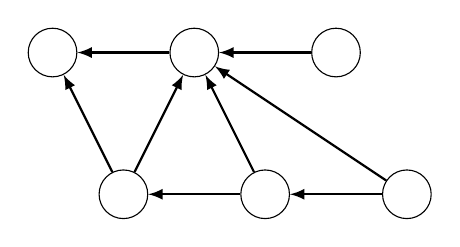
\begin{tikzpicture}[scale=0.9]
\node[draw, circle] (1) at (0,0) {\phantom{0}};
\node[draw, circle] (2) at (2,0) {\phantom{0}};
\node[draw, circle] (3) at (4,0) {\phantom{0}};
\node[draw, circle] (4) at (1,-2) {\phantom{0}};
\node[draw, circle] (5) at (3,-2) {\phantom{0}};
\node[draw, circle] (6) at (5,-2) {\phantom{0}};

\path[draw,thick,->,>=latex] (2) -- (1);
\path[draw,thick,->,>=latex] (3) -- (2);
\path[draw,thick,->,>=latex] (5) -- (4);
\path[draw,thick,->,>=latex] (6) -- (5);
\path[draw,thick,->,>=latex] (4) -- (1);
\path[draw,thick,->,>=latex] (4) -- (2);
\path[draw,thick,->,>=latex] (5) -- (2);
\path[draw,thick,->,>=latex] (6) -- (2);
\end{tikzpicture}
\end{center}
los números de Grundy son los siguientes:
\begin{center}
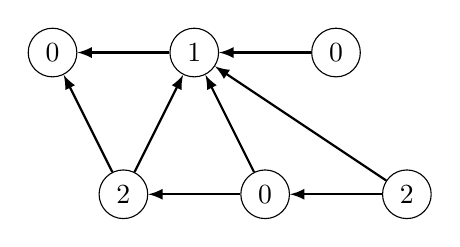
\begin{tikzpicture}[scale=0.9]
\node[draw, circle] (1) at (0,0) {0};
\node[draw, circle] (2) at (2,0) {1};
\node[draw, circle] (3) at (4,0) {0};
\node[draw, circle] (4) at (1,-2) {2};
\node[draw, circle] (5) at (3,-2) {0};
\node[draw, circle] (6) at (5,-2) {2};

\path[draw,thick,->,>=latex] (2) -- (1);
\path[draw,thick,->,>=latex] (3) -- (2);
\path[draw,thick,->,>=latex] (5) -- (4);
\path[draw,thick,->,>=latex] (6) -- (5);
\path[draw,thick,->,>=latex] (4) -- (1);
\path[draw,thick,->,>=latex] (4) -- (2);
\path[draw,thick,->,>=latex] (5) -- (2);
\path[draw,thick,->,>=latex] (6) -- (2);
\end{tikzpicture}
\end{center}
El número de Grundy de un estado perdedor es 0,
y el número de Grundy de un estado ganador es
un número positivo.

El número de Grundy de un estado corresponde a
el número de varas en una pila de nim.
Si el número de Grundy es 0, solo podemos movernos a
estados cuyos números de Grundy sean positivos,
y si el número de Grundy es $x>0$, podemos movernos
a estados cuyos números de Grundy incluyan todos los números
$0,1,\ldots,x-1$.

Como ejemplo, considera un juego donde
los jugadores mueven una figura en un laberinto.
Cada casilla del laberinto es o bien suelo o bien pared.
En cada turno, el jugador tiene que mover
la figura un número
de pasos a la izquierda o hacia arriba.
El ganador del juego es el jugador que
hace la última jugada.

La siguiente imagen muestra un posible estado inicial
del juego, donde @ denota la figura y *
denota una casilla donde puede moverse.

\begin{center}
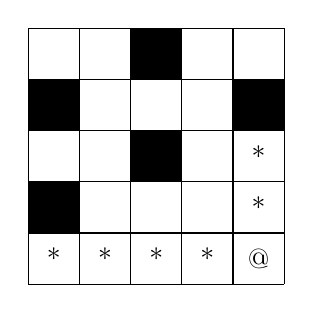
\begin{tikzpicture}[scale=.65]
  \begin{scope}
    \fill [color=black] (0, 1) rectangle (1, 2);
    \fill [color=black] (0, 3) rectangle (1, 4);
    \fill [color=black] (2, 2) rectangle (3, 3);
    \fill [color=black] (2, 4) rectangle (3, 5);
    \fill [color=black] (4, 3) rectangle (5, 4);

    \draw (0, 0) grid (5, 5);
    
    \node at (4.5,0.5) {@};
    \node at (3.5,0.5) {*};
    \node at (2.5,0.5) {*};
    \node at (1.5,0.5) {*};
    \node at (0.5,0.5) {*};
    \node at (4.5,1.5) {*};
    \node at (4.5,2.5) {*};

  \end{scope}

\end{tikzpicture}
\end{center}

Los estados del juego son todos los 
cuadrados del suelo del laberinto.
En el laberinto anterior, los números 
de Grundy son los siguientes:

\begin{center}
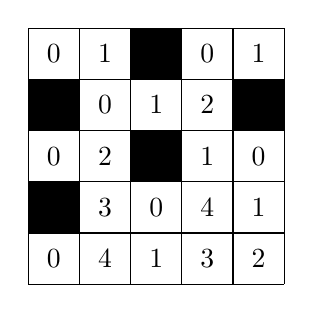
\begin{tikzpicture}[scale=.65]
  \begin{scope}
    \fill [color=black] (0, 1) rectangle (1, 2);
    \fill [color=black] (0, 3) rectangle (1, 4);
    \fill [color=black] (2, 2) rectangle (3, 3);
    \fill [color=black] (2, 4) rectangle (3, 5);
    \fill [color=black] (4, 3) rectangle (5, 4);

    \draw (0, 0) grid (5, 5);
    
    \node at (0.5,4.5) {0};
    \node at (1.5,4.5) {1};
    \node at (2.5,4.5) {};
    \node at (3.5,4.5) {0};
    \node at (4.5,4.5) {1};

    \node at (0.5,3.5) {};
    \node at (1.5,3.5) {0};
    \node at (2.5,3.5) {1};
    \node at (3.5,3.5) {2};
    \node at (4.5,3.5) {};

    \node at (0.5,2.5) {0};
    \node at (1.5,2.5) {2};
    \node at (2.5,2.5) {};
    \node at (3.5,2.5) {1};
    \node at (4.5,2.5) {0};

    \node at (0.5,1.5) {};
    \node at (1.5,1.5) {3};
    \node at (2.5,1.5) {0};
    \node at (3.5,1.5) {4};
    \node at (4.5,1.5) {1};

    \node at (0.5,0.5) {0};
    \node at (1.5,0.5) {4};
    \node at (2.5,0.5) {1};
    \node at (3.5,0.5) {3};
    \node at (4.5,0.5) {2};
  \end{scope}
\end{tikzpicture}
\end{center}

Por lo tanto, cada estado del juego del laberinto
corresponde a un montón en el juego de nim.
Por ejemplo, el número de Grundy para
el cuadrado inferior derecho es 2,
por lo que es un estado ganador.
Podemos llegar a un estado perdedor y
ganar el juego moviendo
ya sea cuatro pasos a la izquierda o
dos pasos hacia arriba.

Tenga en cuenta que a diferencia del juego nim original,
puede ser posible mover a un estado cuyo
número de Grundy es mayor que el número de Grundy
del estado actual.
Sin embargo, el oponente siempre puede elegir una jugada
que cancele esa jugada, por lo que no es posible
escapar de un estado perdedor.

\subsubsection{Subjuegos}

A continuación, asumiremos que nuestro juego consiste
en subjuegos, y en cada turno, el jugador
primero elige un subjuego y luego un movimiento en el subjuego.
El juego termina cuando no es posible realizar ningún movimiento
en ningún subjuego.

En este caso, el número de Grundy de un juego
es la suma nim de los números de Grundy de los subjuegos.
El juego se puede jugar como un juego de nim calculando
todos los números de Grundy para los subjuegos y luego su suma nim.

Como ejemplo, considere un juego que consiste
en tres laberintos.
En este juego, en cada turno, el jugador elige uno
de los laberintos y luego mueve la figura en el laberinto.
Asuma que el estado inicial del juego es el siguiente:

\begin{center}
\begin{tabular}{ccc}
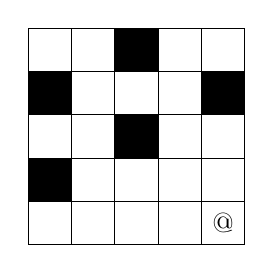
\begin{tikzpicture}[scale=.55]
  \begin{scope}
    \fill [color=black] (0, 1) rectangle (1, 2);
    \fill [color=black] (0, 3) rectangle (1, 4);
    \fill [color=black] (2, 2) rectangle (3, 3);
    \fill [color=black] (2, 4) rectangle (3, 5);
    \fill [color=black] (4, 3) rectangle (5, 4);

    \draw (0, 0) grid (5, 5);

    \node at (4.5,0.5) {@};

    \end{scope}
\end{tikzpicture}
&
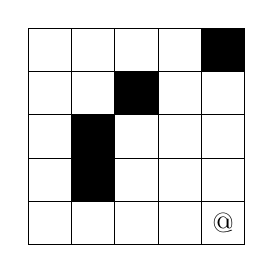
\begin{tikzpicture}[scale=.55]
  \begin{scope}
    \fill [color=black] (1, 1) rectangle (2, 3);
    \fill [color=black] (2, 3) rectangle (3, 4);
    \fill [color=black] (4, 4) rectangle (5, 5);

    \draw (0, 0) grid (5, 5);
    
    \node at (4.5,0.5) {@};

  \end{scope}
\end{tikzpicture}
&
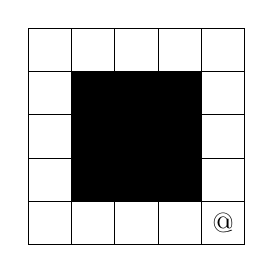
\begin{tikzpicture}[scale=.55]
  \begin{scope}
    \fill [color=black] (1, 1) rectangle (4, 4);

    \draw (0, 0) grid (5, 5);
    
    \node at (4.5,0.5) {@};
  \end{scope}
\end{tikzpicture}
\end{tabular}
\end{center}

Los números de Grundy para los laberintos son los siguientes:

\begin{center}
\begin{tabular}{ccc}
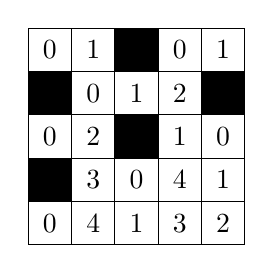
\begin{tikzpicture}[scale=.55]
  \begin{scope}
    \fill [color=black] (0, 1) rectangle (1, 2);
    \fill [color=black] (0, 3) rectangle (1, 4);
    \fill [color=black] (2, 2) rectangle (3, 3);
    \fill [color=black] (2, 4) rectangle (3, 5);
    \fill [color=black] (4, 3) rectangle (5, 4);

    \draw (0, 0) grid (5, 5);

    \node at (0.5,4.5) {0};
    \node at (1.5,4.5) {1};
    \node at (2.5,4.5) {};
    \node at (3.5,4.5) {0};
    \node at (4.5,4.5) {1};

    \node at (0.5,3.5) {};
    \node at (1.5,3.5) {0};
    \node at (2.5,3.5) {1};
    \node at (3.5,3.5) {2};
    \node at (4.5,3.5) {};

    \node at (0.5,2.5) {0};
    \node at (1.5,2.5) {2};
    \node at (2.5,2.5) {};
    \node at (3.5,2.5) {1};
    \node at (4.5,2.5) {0};

    \node at (0.5,1.5) {};
    \node at (1.5,1.5) {3};
    \node at (2.5,1.5) {0};
    \node at (3.5,1.5) {4};
    \node at (4.5,1.5) {1};

    \node at (0.5,0.5) {0};
    \node at (1.5,0.5) {4};
    \node at (2.5,0.5) {1};
    \node at (3.5,0.5) {3};
    \node at (4.5,0.5) {2};
    \end{scope}
\end{tikzpicture}
&
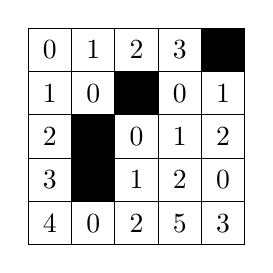
\begin{tikzpicture}[scale=.55]
  \begin{scope}
    \fill [color=black] (1, 1) rectangle (2, 3);
    \fill [color=black] (2, 3) rectangle (3, 4);
    \fill [color=black] (4, 4) rectangle (5, 5);

    \draw (0, 0) grid (5, 5);

    \node at (0.5,4.5) {0};
    \node at (1.5,4.5) {1};
    \node at (2.5,4.5) {2};
    \node at (3.5,4.5) {3};
    \node at (4.5,4.5) {};

    \node at (0.5,3.5) {1};
    \node at (1.5,3.5) {0};
    \node at (2.5,3.5) {};
    \node at (3.5,3.5) {0};
    \node at (4.5,3.5) {1};

    \node at (0.5,2.5) {2};
    \node at (1.5,2.5) {};
    \node at (2.5,2.5) {0};
    \node at (3.5,2.5) {1};
    \node at (4.5,2.5) {2};

    \node at (0.5,1.5) {3};
    \node at (1.5,1.5) {};
    \node at (2.5,1.5) {1};
    \node at (3.5,1.5) {2};
    \node at (4.5,1.5) {0};

    \node at (0.5,0.5) {4};
    \node at (1.5,0.5) {0};
    \node at (2.5,0.5) {2};
    \node at (3.5,0.5) {5};
    \node at (4.5,0.5) {3};
  \end{scope}
\end{tikzpicture}
&
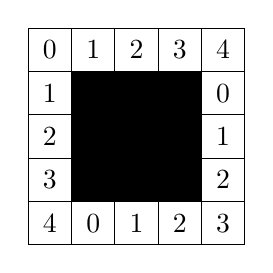
\begin{tikzpicture}[scale=.55]
  \begin{scope}
    \fill [color=black] (1, 1) rectangle (4, 4);

    \draw (0, 0) grid (5, 5);

    \node at (0.5,4.5) {0};
    \node at (1.5,4.5) {1};
    \node at (2.5,4.5) {2};
    \node at (3.5,4.5) {3};
    \node at (4.5,4.5) {4};

    \node at (0.5,3.5) {1};
    \node at (1.5,3.5) {};
    \node at (2.5,3.5) {};
    \node at (3.5,3.5) {};
    \node at (4.5,3.5) {0};

    \node at (0.5,2.5) {2};
    \node at (1.5,2.5) {};
    \node at (2.5,2.5) {};
    \node at (3.5,2.5) {};
    \node at (4.5,2.5) {1};

    \node at (0.5,1.5) {3};
    \node at (1.5,1.5) {};
    \node at (2.5,1.5) {};
    \node at (3.5,1.5) {};
    \node at (4.5,1.5) {2};

    \node at (0.5,0.5) {4};
    \node at (1.5,0.5) {0};
    \node at (2.5,0.5) {1};
    \node at (3.5,0.5) {2};
    \node at (4.5,0.5) {3};
  \end{scope}
\end{tikzpicture}
\end{tabular}
\end{center}

En el estado inicial, la suma nim de los números de Grundy
es $2 \oplus 3 \oplus 3 = 2$, entonces
el primer jugador puede ganar el juego.
Un movimiento óptimo es moverse dos pasos hacia arriba
en el primer laberinto, lo que produce la suma nim
$0 \oplus 3 \oplus 3 = 0$.

\subsubsection{El juego de Grundy}

A veces un movimiento en un juego divide el juego
en subjuegos que son independientes entre sí.
En este caso, el número de Grundy del juego es

\[\textrm{mex}(\{g_1, g_2, \ldots, g_n \}),\]
donde $n$ es el número de posibles movimientos y
\[g_k = a_{k,1} \oplus a_{k,2} \oplus \ldots \oplus a_{k,m},\]
donde el movimiento $k$ genera subjuegos con
números de Grundy $a_{k,1},a_{k,2},\ldots,a_{k,m}$.

\index{El juego de Grundy}

Un ejemplo de tal juego es \key{el juego de Grundy}.
Inicialmente, hay un solo montón que contiene $n$ palitos.
En cada turno, el jugador elige un montón y lo divide
en dos montones no vacíos de modo que los montones
sean de tamaño diferente.
El jugador que realiza el último movimiento gana el juego.

Sea $f(n)$ el número de Grundy de un montón
que contiene $n$ palitos.
El número de Grundy se puede calcular pasando
por todas las formas de dividir el montón en
dos montones.
Por ejemplo, cuando $n=8$, las posibilidades
son $1+7$, $2+6$ y $3+5$, entonces
\[f(8)=\textrm{mex}(\{f(1) \oplus f(7), f(2) \oplus f(6), f(3) \oplus f(5)\}).\]

En este juego, el valor de $f(n)$ se basa en los valores
de $f(1),\ldots,f(n-1)$.
Los casos base son $f(1)=f(2)=0$,
porque no es posible dividir los montones
de 1 y 2 palitos.
Los primeros números de Grundy son:
\[
\begin{array}{lcl}
f(1) & = & 0 \\
f(2) & = & 0 \\
f(3) & = & 1 \\
f(4) & = & 0 \\
f(5) & = & 2 \\
f(6) & = & 1 \\
f(7) & = & 0 \\
f(8) & = & 2 \\
\end{array}
\]
El número de Grundy para $n=8$ es 2,
entonces es posible ganar el juego.
El movimiento ganador es crear montones
$1+7$, porque $f(1) \oplus f(7) = 0$.
